% !TEX TS-program = pdflatex
\documentclass[aspectratio=169]{beamer}
\usepackage[utf8]{inputenc}
\usepackage[T1]{fontenc}
\usetheme{Madrid}
\usecolortheme{seahorse}
\usefonttheme{professionalfonts}
\setbeamertemplate{navigation symbols}{}
\setbeamercovered{transparent}
\setbeamertemplate{itemize items}[circle]
\setbeamertemplate{enumerate items}[default]
\setlength{\parskip}{0.15em}

\definecolor{bepurple}{RGB}{107,63,160}
\definecolor{begold}{RGB}{200,168,75}
\definecolor{beteal}{RGB}{26,122,110}
\definecolor{berust}{RGB}{192,68,42}
\definecolor{beblue}{RGB}{26,74,138}
\definecolor{softpurple}{RGB}{240,232,255}
\definecolor{softgold}{RGB}{255,248,220}
\definecolor{softteal}{RGB}{220,242,240}
\definecolor{softrust}{RGB}{255,235,230}
\setbeamercolor{structure}{fg=beblue}
\setbeamercolor{title}{fg=white,bg=beblue}
\setbeamercolor{frametitle}{fg=beblue}
% Minimal block rendering: regular/example blocks become colored headings (no box)
\setbeamertemplate{block begin}{%
  \par\vspace{0.2ex}%
  \ifx\insertblocktitle\empty\else%
    {\usebeamerfont{block title}\color{beblue}\textbf{\insertblocktitle}}\par\vspace{0.2ex}%
  \fi%
}
\setbeamertemplate{block end}{\par\vspace{0.2ex}}
\setbeamertemplate{block example begin}{%
  \par\vspace{0.2ex}%
  \ifx\insertblocktitle\empty\else%
    {\usebeamerfont{block title}\color{beteal}\textbf{\insertblocktitle}}\par\vspace{0.2ex}%
  \fi%
}
\setbeamertemplate{block example end}{\par\vspace{0.2ex}}
\setbeamertemplate{block alerted begin}{%
  \par\vspace{0.5ex}%
  \begin{beamercolorbox}[sep=0.5ex,rounded=true,shadow=false]{block title alerted}%
    \usebeamerfont{block title}\insertblocktitle%
  \end{beamercolorbox}%
  \nointerlineskip%
  \begin{beamercolorbox}[sep=0.5ex,rounded=true,shadow=false]{block body alerted}%
    \usebeamerfont{block body}%
}
\setbeamertemplate{block alerted end}{\end{beamercolorbox}\par\vspace{0.5ex}}
\setbeamercolor{block title alerted}{fg=white,bg=berust}
\setbeamercolor{block body alerted}{fg=black,bg=berust!8}
\setbeamercolor{alerted text}{fg=berust}

\usepackage{booktabs,amsmath,amssymb,array,multirow,hyperref,colortbl,xcolor}
\usepackage{tikz}
\usepackage{pgfplots}
\pgfplotsset{compat=1.18}
\usetikzlibrary{arrows.meta,positioning,calc,shapes.geometric,patterns}
\hypersetup{colorlinks=true,linkcolor=beblue,urlcolor=beblue}

\title{\textbf{Lecture 1: Foundations of Behavioural Economics}}
\subtitle{Limits of Rationality --- Why the Standard Model Breaks Down}
\author{Prof.\ Muhebullah Karimzada}
\institute{School of Economics, University of Northern British Columbia}
\date{ECON 230 $\cdot$ Introduction to Behavioural Economics $\cdot$ Winter 2027}

\begin{document}

% ============================================================
\begin{frame}[plain]
  \titlepage
\end{frame}

% ============================================================
\begin{frame}{Before We Begin --- A Puzzle}
\note{Run this BEFORE any theory. Collect choices by show of hands. Write results on board. Return to this at slide 9.}
\begin{alertblock}{The Allais Paradox --- Your Turn}
\textbf{Problem A} --- Choose ONE:
\begin{itemize}
  \item Option 1: \$1{,}000{,}000 \textbf{for certain}
  \item Option 2: 89\% chance of \$1M, 10\% chance of \$5M, 1\% chance of \$0
\end{itemize}
\medskip
\textbf{Problem B} --- Choose ONE:
\begin{itemize}
  \item Option 1: 11\% chance of \$1M, 89\% chance of \$0
  \item Option 2: 10\% chance of \$5M, 90\% chance of \$0
\end{itemize}
\end{alertblock}
\medskip
\centering \textbf{Write your choices down. We will return to this in 30 minutes.}
\end{frame}

% ============================================================
\begin{frame}{Course Roadmap --- ECON 230}
\begin{columns}
\column{0.5\textwidth}
\begin{block}{Foundations}
\begin{enumerate}
  \item Limits of Rationality \textcolor{berust}{$\leftarrow$ Today}
  \item Heuristics and Biases
  \item Prospect Theory
\end{enumerate}
\end{block}
\begin{block}{Risk \& Time}
\begin{enumerate}\setcounter{enumi}{3}
  \item Time Inconsistency \& Present Bias
  \item Savings Behaviour
\end{enumerate}
\end{block}
\column{0.5\textwidth}
\begin{block}{Social \& Strategic}
\begin{enumerate}\setcounter{enumi}{5}
  \item Social Preferences
  \item Behavioural Game Theory
\end{enumerate}
\end{block}
\begin{block}{Markets \& Policy}
\begin{enumerate}\setcounter{enumi}{7}
  \item Behavioural Finance
  \item Nudges \& Choice Architecture
  \item Applications \& Policy Design
\end{enumerate}
\end{block}
\end{columns}
\end{frame}

% ============================================================
\section{The Standard Model}
% ============================================================

\begin{frame}{What Does Economics Assume?}
\begin{block}{The Rational Agent}
Standard economics assumes agents are: \textbf{fully rational, perfectly informed, and purely self-interested.}
\end{block}
\begin{itemize}[<+->]
  \item \textbf{Complete preferences:} You can rank \emph{every} possible outcome. No indecision.
  \item \textbf{Transitivity:} If you prefer A to B and B to C, you prefer A to C. Always.
  \item \textbf{Full optimisation:} Given all information, you compute the globally optimal action --- at zero cognitive cost.
  \item \textbf{Bayesian updating:} When new information arrives, you update your beliefs exactly as Bayes' rule dictates.
  \item \textbf{Time consistency:} Your preferences do not change as options approach in time.
\end{itemize}
\pause
\begin{exampleblock}{Why assume this?}
Not because economists think people are robots --- but because this benchmark generates sharp, testable predictions. The question is: \alert{how far does it take us?}
\end{exampleblock}
\end{frame}

% ============================================================
\begin{frame}{Expected Utility Theory}
\note{VNM (1944) is a towering achievement. Make clear: this is the NORMATIVE benchmark --- what a perfectly rational agent SHOULD do. Behavioural economics asks what people ACTUALLY do.}
\begin{block}{Von Neumann \& Morgenstern (1944)}
Under uncertainty, a rational agent maximises:
\[
  EU = \sum_{i} p_i \cdot u(x_i)
\]
where $p_i$ is the probability of outcome $x_i$ and $u(\cdot)$ is a utility function.
\end{block}
\begin{columns}
\column{0.55\textwidth}
\begin{itemize}[<+->]
  \item \textbf{Example:} Gamble A = 50\% chance of \$100, 50\% chance of \$0.
  \item $EU(A) = 0.5 \cdot u(\$100) + 0.5 \cdot u(\$0)$
  \item A \textbf{concave} $u$ captures \alert{risk aversion}: prefer \$50 for sure over the gamble.
  \item Rests on 4 axioms: completeness, transitivity, continuity, \alert{independence}.
  \item \textbf{Violate any axiom} $\Rightarrow$ EU collapses.
\end{itemize}
\column{0.42\textwidth}
\begin{tikzpicture}
\begin{axis}[
  width=\textwidth, height=0.48\textheight,
  xlabel={\small Wealth (\$)},ylabel={\small Utility},
  xmin=0,xmax=110,ymin=0,ymax=115,
  xtick={0,50,100},xticklabels={0,50,100},
  ytick={},yticklabels={},
  axis lines=left,thick,
  title={\small Concave Utility: Risk Aversion}
]
\addplot[color=beblue,very thick,domain=1:110,samples=80]{10*sqrt(x)};
\addplot[color=beteal,dashed,thick] coordinates{(0,70.7)(50,70.7)};
\addplot[color=beteal,dashed,thick] coordinates{(50,0)(50,70.7)};
\addplot[color=berust,dashed,thick] coordinates{(0,0)(100,100)};
\node[font=\tiny,beteal] at (axis cs:72,74) {$u(\$50)$};
\node[font=\tiny,berust] at (axis cs:72,52) {$EU(\text{gamble})$};
\end{axis}
\end{tikzpicture}
\end{columns}
\end{frame}

% ============================================================
\begin{frame}{The Four Axioms in Plain English}
\begin{columns}
\column{0.5\textwidth}
\begin{block}{Completeness}
You can always compare two options. ``I just can't decide'' is not allowed.
\end{block}
\begin{block}{Transitivity}
If $A \succ B$ and $B \succ C$, then $A \succ C$. No preference cycles.
\end{block}
\column{0.5\textwidth}
\begin{block}{Continuity}
Small changes in probability create small changes in preferences. No ``lexicographic'' preferences.
\end{block}
\begin{alertblock}{Independence (The Critical Axiom)}
If $A \succ B$, mixing with $C$ preserves: $(pA + (1-p)C) \succ (pB + (1-p)C)$.
\end{alertblock}
\end{columns}
\textcolor{beteal}{\textbf{Why it matters:}} Independence makes probabilities ``multiply through'' in EU --- and it is precisely what Allais showed \textbf{most people violate systematically}.
\end{frame}

% ============================================================
\begin{frame}{The Power of the Rational Model}
\begin{itemize}[<+->]
  \item \textbf{Nuclear deterrence:} Schelling's (1960) rational-actor analysis of mutually assured destruction.
  \item \textbf{Portfolio theory:} Markowitz (1952) --- diversification as rational risk management. \textit{Nobel 1990.}
  \item \textbf{Auction design:} Milgrom \& Wilson (2020) --- FCC spectrum auctions earned billions for US taxpayers using rational bidding theory.
  \item \textbf{Insurance markets:} Arrow (1963) --- why insurance exists and when it fails.
  \item \textbf{Trade theory:} Comparative advantage, gains from trade --- all built on rational optimisation.
\end{itemize}
\pause
\begin{alertblock}{The Point}
Do NOT dismiss the rational model. It is enormously powerful. Our goal is to understand \alert{where it breaks down} --- and what replaces it there.
\end{alertblock}
\end{frame}

% ============================================================
\section{Evidence Against the Standard Model}
% ============================================================

\begin{frame}{The Allais Paradox --- Back to Your Choices}
\note{Most students choose Option 1 in Problem A and Option 2 in Problem B. Show this is mathematically inconsistent. Allais (1953) won the Nobel Prize partly for this.}
\begin{columns}
\column{0.52\textwidth}
\begin{block}{What Most People Choose}
\begin{itemize}
  \item Problem A: \textbf{Option 1} (certain \$1M)
  \item Problem B: \textbf{Option 2} (10\% chance of \$5M)
\end{itemize}
\end{block}
\begin{alertblock}{The Problem}
Under EU, let $u(0)=0$. Then:
\begin{align*}
A1 \succ A2 &\Rightarrow u(1M) > 0.89\,u(1M) + 0.1\,u(5M)\\
&\Rightarrow 0.11\,u(1M) > 0.1\,u(5M)
\end{align*}
But $B2 \succ B1$ implies the \textbf{opposite}! \alert{Contradiction.}
\end{alertblock}
\column{0.45\textwidth}
\begin{exampleblock}{Allais (1953)}
Maurice Allais presented this to leading economists at a Paris conference. \textbf{Paul Samuelson} (Nobel 1970) initially violated it himself before correcting his answer. ``The Allais Paradox'' has been replicated worldwide across cultures, stake sizes, and expert audiences.
\end{exampleblock}
\vspace{0.5em}
\textcolor{bepurple}{\textbf{The violation of the Independence Axiom is not a mistake --- it is a systematic preference.}}
\end{columns}
\end{frame}

% ============================================================
\begin{frame}{The Ellsberg Paradox (1961)}
\begin{block}{The Setup}
An urn contains 90 balls: 30 are \textcolor{berust}{red}; the remaining 60 are either \textcolor{beblue}{black} or \textcolor{begold}{yellow} in unknown proportions.
\end{block}
\begin{columns}
\column{0.5\textwidth}
\begin{block}{Problem 1: Bet on...}
\begin{itemize}
  \item A: Win \$100 if \textcolor{berust}{red} drawn
  \item B: Win \$100 if \textcolor{beblue}{black} drawn
\end{itemize}
\textit{Most prefer A.}
\end{block}
\begin{block}{Problem 2: Bet on...}
\begin{itemize}
  \item C: Win \$100 if \textcolor{berust}{red} or \textcolor{begold}{yellow}
  \item D: Win \$100 if \textcolor{beblue}{black} or \textcolor{begold}{yellow}
\end{itemize}
\textit{Most prefer D.}
\end{block}
\column{0.47\textwidth}
\begin{alertblock}{The Contradiction}
$A \succ B$ implies $P(\text{red}) > P(\text{black})$. But $D \succ C$ implies $P(\text{black}) > P(\text{red})$. \alert{Violates Savage's Sure-Thing Principle.}
\end{alertblock}
\begin{exampleblock}{Key Insight}
People dislike \textbf{ambiguity} (unknown probabilities) more than \textbf{risk} (known probabilities). This is \alert{ambiguity aversion} --- distinct from risk aversion.
\end{exampleblock}
\end{columns}
\end{frame}

% ============================================================
\begin{frame}{Framing Effects --- The Asian Disease Problem}
\note{Same mathematical outcome, completely different choices. This single result from Kahneman \& Tversky (1981) undermines the idea that preferences are defined over final outcomes.}
\begin{columns}
\column{0.5\textwidth}
\begin{block}{Gain Frame}
A disease will kill 600 people. Choose:
\begin{itemize}
  \item A: 200 people will be \textbf{saved}
  \item B: 1/3 prob all 600 saved; 2/3 prob nobody saved
\end{itemize}
\textcolor{beteal}{\textbf{72\% choose A.}}
\end{block}
\column{0.5\textwidth}
\begin{alertblock}{Loss Frame}
Same disease. Choose:
\begin{itemize}
  \item C: 400 people will \textbf{die}
  \item D: 1/3 prob nobody dies; 2/3 prob 600 die
\end{itemize}
\textcolor{berust}{\textbf{78\% choose D.}}
\end{alertblock}
\end{columns}
\medskip
\begin{block}{A = C and B = D --- Mathematically Identical}
Under EU, the same person should choose either $\{A, C\}$ or $\{B, D\}$. Yet most choose $\{A, D\}$.
\textit{Kahneman \& Tversky, 1981, Science.} Replicated in 50+ countries.
\end{block}
\end{frame}

% ============================================================
\begin{frame}{Loss Aversion --- The Asymmetry of Pain}
\begin{columns}
\column{0.53\textwidth}
\begin{block}{The Finding}
\textbf{Losses loom approximately 2--2.5 times larger than equivalent gains.} \\[0.5em]
$\lambda \approx 2.25$ \quad (Tversky \& Kahneman, 1992)
\end{block}
\begin{itemize}[<+->]
  \item Ask: ``Would you accept a 50/50 bet to win \$150 or lose \$100?'' Most say \textbf{no}.
  \item EU with a concave function cannot explain this for small stakes.
  \item Consumer panel study (butter): $\lambda \approx 2.4$ (Hardie, Johnson \& Fader, 1993).
  \item Labour market: workers resist nominal wage cuts even when real wages are falling (Akerlof et al., 1996).
\end{itemize}
\column{0.44\textwidth}
\begin{tikzpicture}
\begin{axis}[
  width=\textwidth, height=0.6\textheight,
  xlabel={\small Outcome},ylabel={\small Subjective Value},
  xmin=-110,xmax=110,ymin=-130,ymax=80,
  axis lines=center,tick style={draw=none},
  xtick={-100,-50,0,50,100},
  xticklabels={\small$-100$,\small$-50$,,\small$50$,\small$100$},
  ytick={},yticklabels={},
  title={\small S-Shaped Value Function (Preview)}
]
\addplot[beteal,very thick,domain=0.5:100,samples=80]{45*(x/50)^0.88};
\addplot[berust,very thick,domain=-100:-0.5,samples=80]{-2.25*45*((-x)/50)^0.88};
\addplot[black,only marks,mark=*,mark size=2pt] coordinates{(0,0)};
\node[font=\scriptsize,right] at (axis cs:3,5){Reference};
\end{axis}
\end{tikzpicture}
\end{columns}
\end{frame}

% ============================================================
\begin{frame}{Present Bias Evidence}
\begin{block}{Thaler (1981) --- The Declining Discount Rate}
Participants asked: ``What amount would make you indifferent between receiving it now vs.\ later?''
\end{block}
\begin{center}
\begin{tabular}{lccc}
\toprule
 & \textbf{Delay: 1 month} & \textbf{Delay: 1 year} & \textbf{Delay: 10 years}\\
\midrule
\$15 now $\to$ \$X later & \$20 & \$50 & \$100\\
\textit{Implied annual rate} & \textit{345\%} & \textit{120\%} & \textit{19\%}\\
\bottomrule
\end{tabular}
\end{center}
\begin{alertblock}{The Problem}
Standard exponential discounting predicts a \textbf{constant} annual discount rate. But observed rates \textbf{decline sharply} with the delay horizon. This generates \alert{time inconsistency}: preferences reverse as the future becomes the present.
\end{alertblock}
\pause
\textcolor{bepurple}{\textbf{Consequence:}} ``I'll start saving next month'' --- said every month for 20 years.
\end{frame}

% ============================================================
\begin{frame}{Overconfidence --- The Evidence}
\begin{columns}
\column{0.53\textwidth}
\begin{itemize}[<+->]
  \item \textbf{Driving:} 93\% of US drivers rate themselves ``above average'' (Svenson, 1981). \textit{Impossible by definition.}
  \item \textbf{Teaching:} 94\% of professors at one US university rated themselves above-average teachers (Cross, 1977).
  \item \textbf{Exams:} Students predict 72\% average; actual = 67\% (Dunning et al., 2003).
  \item \textbf{Investments:} Men trade 45\% more than women; earn 1.4\% less/year (Barber \& Odean, 2001).
  \item \textbf{Projects:} Planning fallacy --- Sydney Opera House budgeted \$7M, cost \$102M.
\end{itemize}
\column{0.44\textwidth}
\begin{tikzpicture}
\begin{axis}[
  width=\textwidth,height=0.6\textheight,
  xlabel={\small Actual Driving Skill (Percentile)},
  ylabel={\small Self-Rated Skill},
  xmin=0,xmax=100,ymin=0,ymax=100,
  axis lines=left,
  title={\small Overconfidence in Driving}
]
\addplot[black,dashed,domain=0:100]{x};
\addplot[berust,thick,domain=0:100]{20+0.6*x};
\node[font=\tiny,berust,rotate=25] at (axis cs:60,60){\textbf{Actual ratings}};
\node[font=\tiny,black,rotate=45] at (axis cs:70,75){\textbf{Calibrated}};
\end{axis}
\end{tikzpicture}
\end{columns}
\end{frame}

% ============================================================
\section{Bounded Rationality}
% ============================================================

\begin{frame}{Herbert Simon --- Bounded Rationality}
\note{Simon (1978 Nobel) is the founding figure. Key message: people are rational BUT within limits. This is the foundational insight of behavioural economics. Not irrational -- boundedly rational.}
\begin{columns}
\column{0.6\textwidth}
\begin{block}{Simon (1955)}
``A wealth of information creates a poverty of attention.''
\end{block}
\begin{itemize}[<+->]
  \item People intend to be rational but are constrained by:
  \begin{enumerate}
    \item \textbf{Cognitive limits:} finite working memory, attention, processing speed.
    \item \textbf{Information limits:} incomplete, costly to gather.
    \item \textbf{Time limits:} real decisions have deadlines.
  \end{enumerate}
  \item \textbf{Satisficing, not optimising:} Search until you find an option above your aspiration level --- then \alert{stop}. (``Good enough.'')
  \item \textbf{Heuristics:} Mental shortcuts substitute for full computation. Often effective; sometimes systematically wrong.
\end{itemize}
\column{0.37\textwidth}
\begin{tikzpicture}
\begin{axis}[
  width=\textwidth,height=0.6\textheight,
  xlabel={\small Options Searched},
  ylabel={\small Option Quality},
  xmin=0,xmax=10,ymin=0,ymax=10,
  axis lines=left,
  title={\small Satisficing vs Optimising}
]
\addplot[beblue,dashed,thick] coordinates{(0,9)(10,9)};
\addplot[begold,dashed,thick] coordinates{(0,6)(10,6)};
\node[font=\tiny,beblue] at (axis cs:6.8,9.4) {Optimum};
\node[font=\tiny,begold!80!black] at (axis cs:6.8,6.4) {Aspiration};
\addplot[only marks,mark=*,berust,mark size=3pt] coordinates{(1,3)(2,4)(3,6.5)(4,5)(5,7)(6,8)(7,6)(8,9)};
\draw[->,very thick,berust] (axis cs:3,6.5) -- (axis cs:3,7) node[above,font=\tiny,berust]{\textbf{STOP}};
\end{axis}
\end{tikzpicture}
\end{columns}
\end{frame}

% ============================================================
\begin{frame}{The Paradox of Choice}
\begin{columns}
\column{0.5\textwidth}
\begin{exampleblock}{The Jam Study (Iyengar \& Lepper, 2000)}
\begin{itemize}
  \item \textbf{24-jam display:} 60\% of shoppers stopped; \textbf{3\%} bought.
  \item \textbf{6-jam display:} 40\% stopped; \textbf{30\%} bought.
  \item \textit{More choice $\Rightarrow$ less action and less satisfaction.}
\end{itemize}
\end{exampleblock}
\begin{exampleblock}{Canadian Context}
Choi et al.\ (2009): Canadians offered \textbf{more mutual fund options} in their RRSP contribute \textbf{less} and choose \textbf{worse} options. Choice overload is real in Canadian retirement savings.
\end{exampleblock}
\column{0.47\textwidth}
\begin{tikzpicture}
\begin{axis}[
  width=\textwidth,height=0.6\textheight,
  ybar,bar width=0.5cm,
  xlabel={\small Display Size},ylabel={\small \% Who Purchased},
  symbolic x coords={6 jams,24 jams},
  xtick=data,ymin=0,ymax=35,
  nodes near coords,
  title={\small Jam Study Results}
]
\addplot[fill=beteal!70] coordinates{(6 jams,30)(24 jams,3)};
\end{axis}
\end{tikzpicture}
\end{columns}
\end{frame}

% ============================================================
\begin{frame}{System 1 vs System 2 (Kahneman, 2011)}
\begin{columns}
\column{0.47\textwidth}
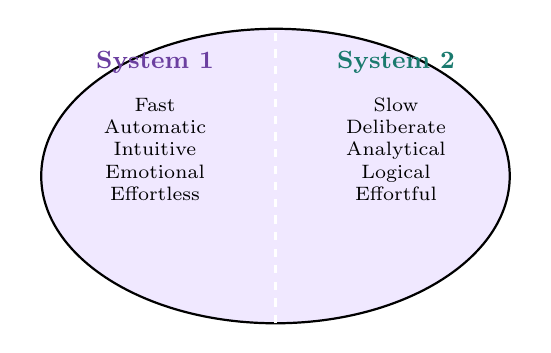
\begin{tikzpicture}[scale=0.85]
\draw[thick,fill=softpurple] (0,0) ellipse (3.5cm and 2.2cm);
\draw[thick,white,dashed] (0,-2.2) -- (0,2.2);
\node[bepurple,font=\bfseries\small] at (-1.8,1.7) {System 1};
\node[font=\scriptsize,text width=3cm,align=center] at (-1.8,0.4)
  {Fast \\ Automatic \\ Intuitive \\ Emotional \\ Effortless};
\node[beteal,font=\bfseries\small] at (1.8,1.7) {System 2};
\node[font=\scriptsize,text width=3cm,align=center] at (1.8,0.4)
  {Slow \\ Deliberate \\ Analytical \\ Logical \\ Effortful};
\end{tikzpicture}
\column{0.5\textwidth}
\begin{alertblock}{The Bat-and-Ball Problem}
A bat and ball cost \$1.10 together. The bat costs \$1.00 more than the ball. How much does the ball cost?
\end{alertblock}
\pause
\begin{block}{System 1 says: \$0.10. \alert{Wrong.}}
Correct answer: \$0.05.\\
\textit{If ball = \$0.10, bat = \$1.10, total = \$1.20. Contradiction.}
\end{block}
\textbf{90\% of people give the wrong answer.} Even Harvard, MIT and Princeton students: 56\% wrong (Frederick, 2005).
\end{columns}
\end{frame}

% ============================================================
\section{In-Class Game: The CRT Test}
% ============================================================

\begin{frame}[t]{[GAME] Cognitive Reflection Test}
\note{Give students EXACTLY 2 minutes, no calculators, no talking. Collect answers on a show of hands after revealing each correct answer. The power of this exercise is seeing how many smart students get these wrong.}
\begin{alertblock}{Rules: 2 minutes, write your answers now, no calculators}
\textbf{Q1.} A bat and a ball cost \$1.10 in total. The bat costs \$1.00 more than the ball. How much does the ball cost? \\[0.4em]
\textbf{Q2.} If it takes 5 machines 5 minutes to make 5 widgets, how long would it take 100 machines to make 100 widgets? \\[0.4em]
\textbf{Q3.} In a lake, a patch of lily pads doubles in size every day. After 48 days the lake is half full. After how many days is the lake completely full?
\end{alertblock}
\medskip
\centering \textit{Answers revealed on next slide...}
\end{frame}

% ============================================================
\begin{frame}{CRT Results and Discussion}
\begin{columns}
\column{0.45\textwidth}
\begin{block}{Answers}
\begin{itemize}
  \item \textbf{Q1:} \$0.05 \textit{(not \$0.10)}
  \item \textbf{Q2:} 5 minutes \textit{(not 100)}
  \item \textbf{Q3:} 49 days \textit{(not 24)}
\end{itemize}
\end{block}
\begin{tikzpicture}
\begin{axis}[
  width=\textwidth,height=0.45\textheight,
  ybar,bar width=0.45cm,symbolic x coords={MIT,Princeton,UNBC avg},
  xtick=data,ymin=0,ymax=100,ylabel={\small \% All 3 Correct},
  nodes near coords,
  title={\small CRT Scores by Group (Frederick 2005)}
]
\addplot[fill=beblue!70] coordinates{(MIT,48)(Princeton,56)(UNBC avg,25)};
\end{axis}
\end{tikzpicture}
\column{0.52\textwidth}
\begin{itemize}[<+->]
  \item Only \textbf{17\%} of US college students get all 3 correct (Frederick, 2005).
  \item MIT: 48\%. Princeton: 56\%.
  \item \textbf{System 1 hijacks System 2} even for intelligent people under time pressure.
  \item Low CRT scores predict: higher present bias, more overconfidence, lower savings rates, poorer financial literacy.
  \item \textit{This is not about intelligence. It's about cognitive engagement.}
\end{itemize}
\end{columns}
\end{frame}

% ============================================================
\begin{frame}{[GAME] Anchoring in Action}
\note{Divide the class in half using the seating arrangement. Each half gets a different anchor question. Collect estimates, compute means, reveal the anchor's effect. Correct answer: Canada population = approximately 40.5 million in 2024 (Statistics Canada).}
\begin{columns}
\column{0.48\textwidth}
\begin{block}{Group A (Left Side)}
Is the population of Canada \textbf{more or less than 10 million}? What is your best estimate of Canada's population?
\end{block}
\column{0.48\textwidth}
\begin{alertblock}{Group B (Right Side)}
Is the population of Canada \textbf{more or less than 100 million}? What is your best estimate of Canada's population?
\end{alertblock}
\end{columns}
\medskip
\begin{block}{Expected Results (Tversky \& Kahneman 1974 design)}
\begin{itemize}
  \item Group A mean estimate: $\approx$ 22--28 million
  \item Group B mean estimate: $\approx$ 40--55 million
  \item \textbf{Correct answer: approximately 40.5 million (Statistics Canada, 2024)}
  \item The \alert{irrelevant} anchor number shifts estimates by 30--50\%.
\end{itemize}
\end{block}
\end{frame}

% ============================================================
\section{Why This Matters}
% ============================================================

\begin{frame}{Markets Do Not Fix Irrational Behaviour}
\begin{itemize}[<+->]
  \item \textbf{Traditional argument:} Markets select against irrational agents --- they lose money and exit.
  \item \textbf{Counter-argument 1 (DeLong et al., 1990):} Limits of arbitrage. Rational traders cannot always profit from others' mistakes --- mispricing can persist or worsen before correcting.
  \item \textbf{Counter-argument 2:} When errors are \alert{correlated} (everyone makes the same mistake), they don't cancel --- they amplify. Example: 2008 financial crisis --- sophisticated institutions all made the same overconfidence mistake simultaneously.
  \item \textbf{Counter-argument 3:} Noise traders can \textit{earn higher expected returns} than rational arbitrageurs if their sentiment risk is priced (DeLong et al., 1990).
\end{itemize}
\pause
\begin{alertblock}{Bottom Line}
Markets reduce but do not eliminate the consequences of systematic cognitive errors.
\end{alertblock}
\end{frame}

% ============================================================
\begin{frame}{The Cost of Cognitive Bias --- Real Data}
\begin{columns}
\column{0.5\textwidth}
\begin{itemize}
  \item \textbf{\$80--100 billion:} Annual cost to US households from investment mistakes (Choi et al., 2010).
  \item \textbf{75\%:} Share of credit card debt explained by present bias (Laibson et al., 2001).
  \item \textbf{1.4\%/year:} Lower net returns from male overconfidence in trading (Barber \& Odean, 2001).
  \item \textbf{27\%:} Canadians who contributed to RRSPs in 2022 --- despite average unused room of \$25{,}000+ (Statistics Canada).
\end{itemize}
\column{0.47\textwidth}
\begin{tikzpicture}
\begin{axis}[
  width=\textwidth,height=0.65\textheight,
  xbar,bar width=0.45cm,
  xlabel={\small Annual Cost (\$B, USA)},
  symbolic y coords={Excess Trading,Credit Card Debt,Undersaving,Total Mistakes},
  ytick=data,
  xmin=0,xmax=110,
  nodes near coords,
  title={\small Annual Costs of Bias (USA)}
]
\addplot[fill=berust!70] coordinates{(10,Excess Trading)(25,Credit Card Debt)(65,Undersaving)(100,Total Mistakes)};
\end{axis}
\end{tikzpicture}
\end{columns}
\end{frame}

% ============================================================
\begin{frame}{Canadian Context --- Savings \& Bias}
\begin{columns}
\column{0.5\textwidth}
\begin{block}{Canadian Savings Data (Statistics Canada, 2022--2024)}
\begin{itemize}
  \item Only \textbf{27\%} of eligible Canadians contributed to RRSPs in 2022.
  \item Median unused RRSP room: \textbf{\$25{,}000+} per filer.
  \item \textbf{47\%} of Canadians live paycheque-to-paycheque (FP Canada, 2023).
  \item Average credit card debt: \textbf{\$4{,}200} at 19.99\% APR (Equifax, 2023).
\end{itemize}
\end{block}
\begin{exampleblock}{}
93\% of Canadians \textit{know} RRSPs exist. The problem is not information --- it is \alert{present bias}.
\end{exampleblock}
\column{0.47\textwidth}
\begin{tikzpicture}
\begin{axis}[
  width=\textwidth,height=0.65\textheight,
  ybar,bar width=0.5cm,
  ylabel={\small \% of Canadians},
  symbolic x coords={RRSP Contributors,Paycheque to Paycheque,No Savings at All},
  xtick=data,
  x tick label style={font=\tiny,rotate=20,anchor=east},
  ymin=0,ymax=60,nodes near coords,
  title={\small Canadian Financial Health (2022--23)}
]
\addplot[fill=beblue!70] coordinates{(RRSP Contributors,27)(Paycheque to Paycheque,47)(No Savings at All,41)};
\end{axis}
\end{tikzpicture}
\end{columns}
\end{frame}

% ============================================================
\begin{frame}{Three Approaches to Economic Policy}
\begin{center}
\begin{tabular}{p{2.5cm}p{3cm}p{3cm}p{3.5cm}}
\toprule
\textbf{Approach} & \textbf{Assumption} & \textbf{Policy Tool} & \textbf{Example}\\
\midrule
\textbf{Standard Econ} & Full rationality & Prices, information & Carbon tax, calorie labels\\[0.5em]
\rowcolor{softpurple}
\textbf{Behavioural} & Bounded rationality & Nudges, defaults, commitment & Auto-enrolment, SMarT\\[0.5em]
\textbf{Hard Paternalism} & Irrationality & Mandates, bans & Helmet laws, sugar bans\\
\bottomrule
\end{tabular}
\end{center}
\medskip
\begin{exampleblock}{The Behavioural Insight}
Behavioural policy does not replace standard policy --- it \alert{complements} it by working with cognitive architecture, not against it.
\end{exampleblock}
\end{frame}

% ============================================================
\section{History \& Nobel Prizes}
% ============================================================

\begin{frame}{A Brief History of Behavioural Economics}
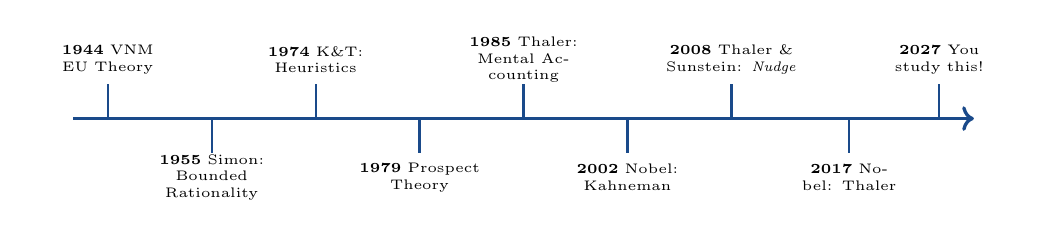
\begin{tikzpicture}[scale=0.88,every node/.style={font=\tiny,align=center,text width=1.8cm}]
  \draw[->,very thick,beblue] (0,0) -- (13,0);
  % Above-timeline items
  \draw[thick,beblue] (0.5,0) -- (0.5,0.5);
  \node at (0.5,0.85) {\textbf{1944} VNM EU Theory};
  \draw[thick,beblue] (3.5,0) -- (3.5,0.5);
  \node at (3.5,0.85) {\textbf{1974} K\&T: Heuristics};
  \draw[thick,beblue] (6.5,0) -- (6.5,0.5);
  \node at (6.5,0.85) {\textbf{1985} Thaler: Mental Accounting};
  \draw[thick,beblue] (9.5,0) -- (9.5,0.5);
  \node at (9.5,0.85) {\textbf{2008} Thaler \& Sunstein: \textit{Nudge}};
  \draw[thick,beblue] (12.5,0) -- (12.5,0.5);
  \node at (12.5,0.85) {\textbf{2027} You study this!};
  % Below-timeline items
  \draw[thick,beblue] (2.0,0) -- (2.0,-0.5);
  \node at (2.0,-0.85) {\textbf{1955} Simon: Bounded Rationality};
  \draw[thick,beblue] (5.0,0) -- (5.0,-0.5);
  \node at (5.0,-0.85) {\textbf{1979} Prospect Theory};
  \draw[thick,beblue] (8.0,0) -- (8.0,-0.5);
  \node at (8.0,-0.85) {\textbf{2002} Nobel: Kahneman};
  \draw[thick,beblue] (11.2,0) -- (11.2,-0.5);
  \node at (11.2,-0.85) {\textbf{2017} Nobel: Thaler};
\end{tikzpicture}
\begin{exampleblock}{Key Figures}
\textbf{Herbert Simon} (Nobel 1978) $\cdot$ \textbf{Daniel Kahneman} (Nobel 2002) $\cdot$ \textbf{Vernon Smith} (Nobel 2002) $\cdot$ \textbf{Richard Thaler} (Nobel 2017)
\end{exampleblock}
\end{frame}

% ============================================================
\begin{frame}{Methods in Behavioural Economics}
\begin{itemize}[<+->]
  \item \textbf{Laboratory experiments:} Controlled environment, randomisation, replication. Trade-off: external validity.
  \item \textbf{Field experiments:} Real-world randomised controlled trials (RCTs). ``Nudge units'' run these in governments.
  \item \textbf{Natural experiments:} Exploit exogenous variation. Organ donation law changes, pension regulation changes.
  \item \textbf{Surveys:} Elicit stated preferences, beliefs, and time preferences. Canadian Survey of Financial Security (Statistics Canada).
  \item \textbf{Revealed preference data:} Transaction records, administrative data, scanner data.
  \item \textbf{Neuroeconomics:} fMRI shows neural correlates of loss aversion, time discounting, social preferences.
\end{itemize}
\end{frame}

% ============================================================
\begin{frame}{The Equity Premium Puzzle --- Preview}
\begin{block}{Mehra \& Prescott (1985)}
US stocks have returned $\approx 6\%$ more per year than bonds since 1871. To justify this within the EU framework, the coefficient of relative risk aversion would need to be $\gamma > 30$ --- \textit{implausibly high.}
\end{block}
\begin{exampleblock}{Behavioural Explanation (Benartzi \& Thaler, 1995)}
If investors are loss averse ($\lambda = 2.25$) and evaluate their portfolio \textbf{annually}, the required equity premium is exactly $\approx 6\%$. The puzzle dissolves with myopic loss aversion.
\end{exampleblock}
\begin{tikzpicture}
\begin{axis}[
  width=0.8\textwidth,height=0.35\textheight,
  xlabel={\small Year},ylabel={\small Cumulative Value (\$)},
  title={\small \$1 Invested in 1871: Stocks vs Bonds (USA)},
  xmin=1870,xmax=2020,ymin=0,ymax=600,
  axis lines=left,legend pos=north west
]
\addplot[beteal,thick,domain=1871:2020,samples=100]{exp((x-1871)*0.063)};
\addplot[berust,thick,domain=1871:2020,samples=100]{exp((x-1871)*0.010)};
\legend{\small Stocks (6.3\%/yr),\small Bonds (1.0\%/yr)}
\end{axis}
\end{tikzpicture}
\end{frame}

% ============================================================
\begin{frame}{Discussion Questions}
\begin{enumerate}
  \item[\textcolor{bepurple}{Q1.}] ``Is it fair to call someone \textit{irrational} when they make a systematic mistake? Who decides what the \textit{right} answer is?''
  \medskip
  \item[\textcolor{beteal}{Q2.}] ``If people aren't fully rational, does this mean governments \textit{should} decide for them? Or does government face the same cognitive limits?''
  \medskip
  \item[\textcolor{berust}{Q3.}] ``Can you think of a decision you made recently that might have violated transitivity, independence, or consistency? Did you feel irrational at the time?''
\end{enumerate}
\medskip
\begin{block}{Think--Pair--Share (3 minutes)}
Discuss Q1 with a neighbour. One person will be asked to share.
\end{block}
\end{frame}

% ============================================================
\begin{frame}{Key Takeaways --- Lecture 1}
\begin{itemize}
  \item[\textcolor{beteal}{\checkmark}] \textbf{Standard model:} rational agents maximise expected utility; four axioms underpin it.
  \item[\textcolor{beteal}{\checkmark}] \textbf{Evidence against:} Allais paradox (independence), Ellsberg (ambiguity), framing effects, loss aversion, overconfidence.
  \item[\textcolor{beteal}{\checkmark}] \textbf{Bounded rationality (Simon):} people intend to be rational but are cognitively, informationally, and temporally constrained.
  \item[\textcolor{beteal}{\checkmark}] \textbf{Satisficing:} search until ``good enough''; heuristics substitute for full optimisation.
  \item[\textcolor{beteal}{\checkmark}] \textbf{Two systems:} fast, intuitive System 1 often overrides deliberate System 2.
  \item[\textcolor{beteal}{\checkmark}] \textbf{Errors are systematic and predictable} $\Rightarrow$ economically important $\Rightarrow$ addressable by policy.
\end{itemize}
\medskip
\begin{alertblock}{The Central Insight of This Course}
People are not irrational. They are \textit{intentionally rational} --- but cognitively constrained. Understanding those constraints is where behavioural economics begins.
\end{alertblock}
\end{frame}

% ============================================================
\begin{frame}{Further Reading}
\begin{itemize}
  \item Kahneman, D.\ (2011). \textit{Thinking, Fast and Slow}. Farrar, Straus \& Giroux. \textcolor{bepurple}{\textbf{Essential.}}
  \item Thaler, R.\ \& Sunstein, C.\ (2008). \textit{Nudge}. Yale University Press.
  \item Ariely, D.\ (2008). \textit{Predictably Irrational}. HarperCollins.
  \item Camerer, C., Loewenstein, G.\ \& Rabin, M.\ (2004). \textit{Advances in Behavioral Economics}. Princeton University Press. \textcolor{bepurple}{\textbf{Academic reference.}}
  \item Tversky, A.\ \& Kahneman, D.\ (1974). Judgment under uncertainty: Heuristics and biases. \textit{Science}, 185, 1124--1131.
  \item Von Neumann, J.\ \& Morgenstern, O.\ (1944). \textit{Theory of Games and Economic Behavior}. Princeton.
\end{itemize}
\medskip\textcolor{beblue}{\textbf{Next:}} \textbf{Lecture 2: Heuristics and Biases} --- We drill deeper into the specific mental shortcuts that cause systematic errors: representativeness, availability, anchoring, confirmation bias, and overconfidence.
\end{frame}

\end{document}
